
\section{\engt{Lesson 3: LED Cube Construction} \nedt{Les 3: LED Cube constructie}}

\subsection{\engt{Layout breadboard}  \nedt{Opstelling schakelbord}}

\eng{We have all the necessary basis to start with making our Fe Cube. We start with putting all components on the breadboard. Then we test it with a program which is our previous RGB LED sketch adapted to the cube. Only when we have verified all works will we start the actual construction.

So, put following components in front of you:
\begin{enumerate}
 \item Your breadboard
 \item 9 RGB-LED (we assume common cathode in the following)
 \item 3 NPN (2N3904 normally)
 \item 9 220 $\Omega$ resistors
 \item many wires.
\end{enumerate}
First, put the RGB-LED on the board, connect the color pins with each other via wires, and connect the common cathode via a resistor to another line, see Fig.~\ref{f:lesson3_bb1}.

Connect then the resistors to pins 1 to 9. These are the pins that will feed the LED. So for a common cathode, these pins on \ardo{HIGH} will make the LED burn. Put the 3 NPN on the board. The color wire goes to the Emitter side (-) of the NPN for common cathode LED. The Colector side (+) goes to the Volt line of your breadboard. The Volt line of the breadboard goes to a 5V pin on the Arduino.

The Base leg of the NPN will control if the NPN junction is open or not. We will use pins 10, 11, 12 to control this. Your entire wiring should look like Fig.~\ref{f:lesson3_bb2}.
}

\ned{We hebben alles gezien om aan onze Fe Kubus te beginnen. We starten met alle componenten op het schakelbord te zetten. Dan testen we de schakeling met een programma die onze vorige RGB LED schets is aangepast voor de kubus. Alleen als we zeker zijn dat alles werkt zullen we de effectieve constructie doen.

Plaats dus de volgende componenten voor jou:
\begin{enumerate}
 \item Jouw schakelbord
 \item 9 RGB-LED (we veronderstellen gemeenschappelijke kathode in wat volgt)
 \item 3 NPN (2N3904 normaal)
 \item 9 220 $\Omega$ weerstanden
 \item veel draden.
\end{enumerate}
Begin met de RGB-LED op je bord te zetten, verbindt de kleurpinnen met elkaar via draden, en connecteer de gemeenschappelijke kathode via een weerstand naar een andere lijn op je bord, zie Fig.~\ref{f:lesson3_bb1}.

Verbind nu de weerstanden met pinnen 1 tot 9. Deze pinnen zullen de LED van stroom voorzien. Dus, voor een gemeenschappelijke kathode zullen we deze pinnen op \ardo{HIGH} zetten om de LED te doen branden. Plaats dan de 3 NPN op het bord. De draden van een kleur gaan naar de Emitter zijde (-) van de NPN voor gemeenschappelijke kathode LEDs. De Collector zijde (+) gaat naar de Voltage lijn op je schakelbord. Deze Voltage lijn gaat dan naar een 5V pin op de Arduino.

Het Basis been van de NPN zal bepalen of de NPN junctie open is of niet. We zullen pinnen 10, 11, 12 gebruiken voor dit been. Je volledige schakeling zou er moeten uitzien als Fig.~\ref{f:lesson3_bb2}.
}

\begin{figure}
  \centering
  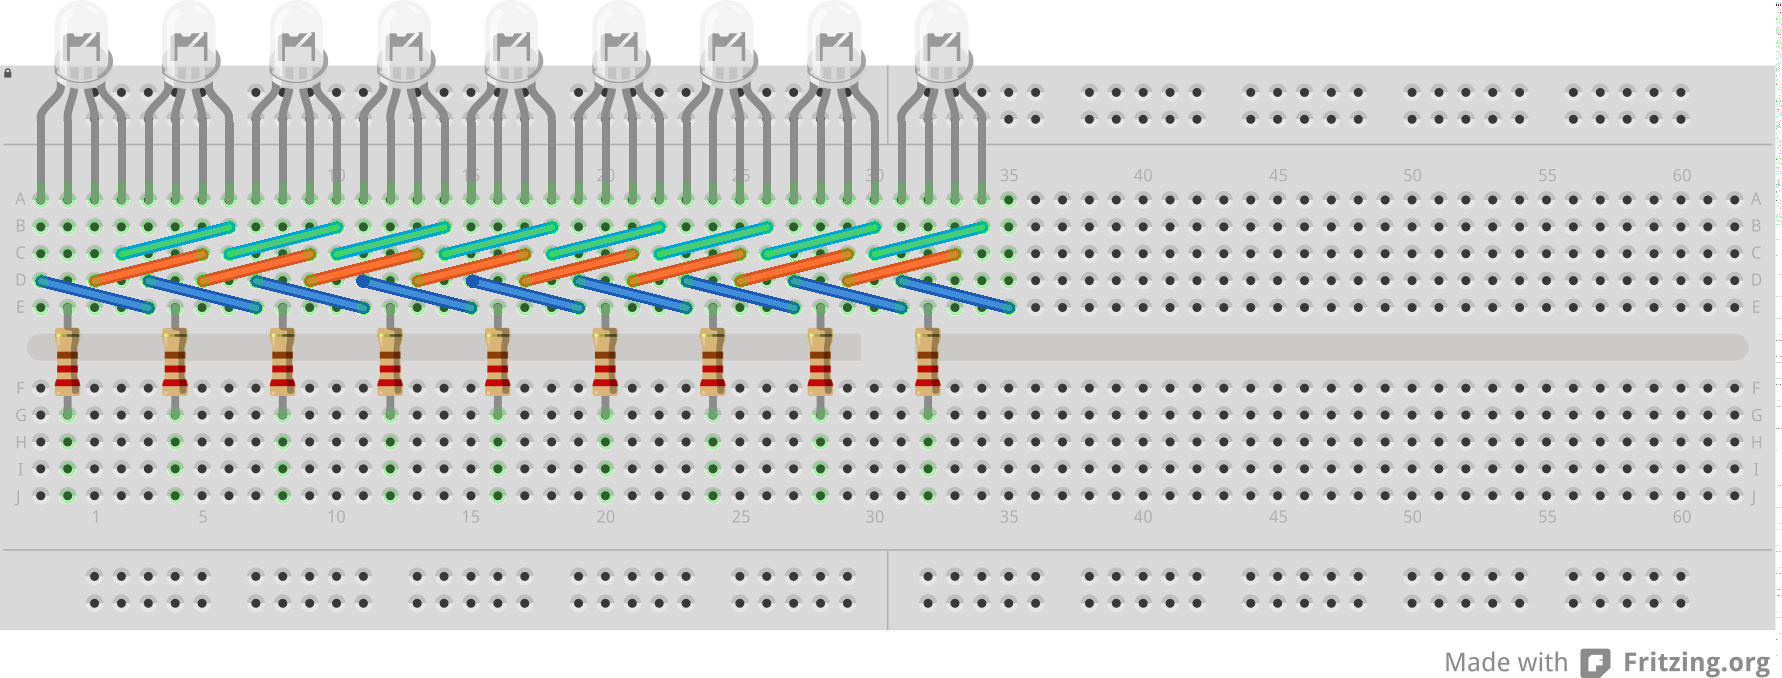
\includegraphics[width=11cm]{img/05_fecube_01_bb.png} 
\caption{\engt{Put the 9 LED on the board. Connect all equal colors to each other. The common cathode or anode goes with a 220 $\Omega$ resistor to a new line} \nedt{Plaats de 9 LED op het bord. Connecteer alle gelijke kleuren met elkaar. De gemeenschappelijke kathode of anode gaat met een 220 $\Omega$ weerstand naar een nieuwe lijn.}}
\label{f:lesson3_bb1}.
\end{figure}
%
\begin{figure}
  \centering
  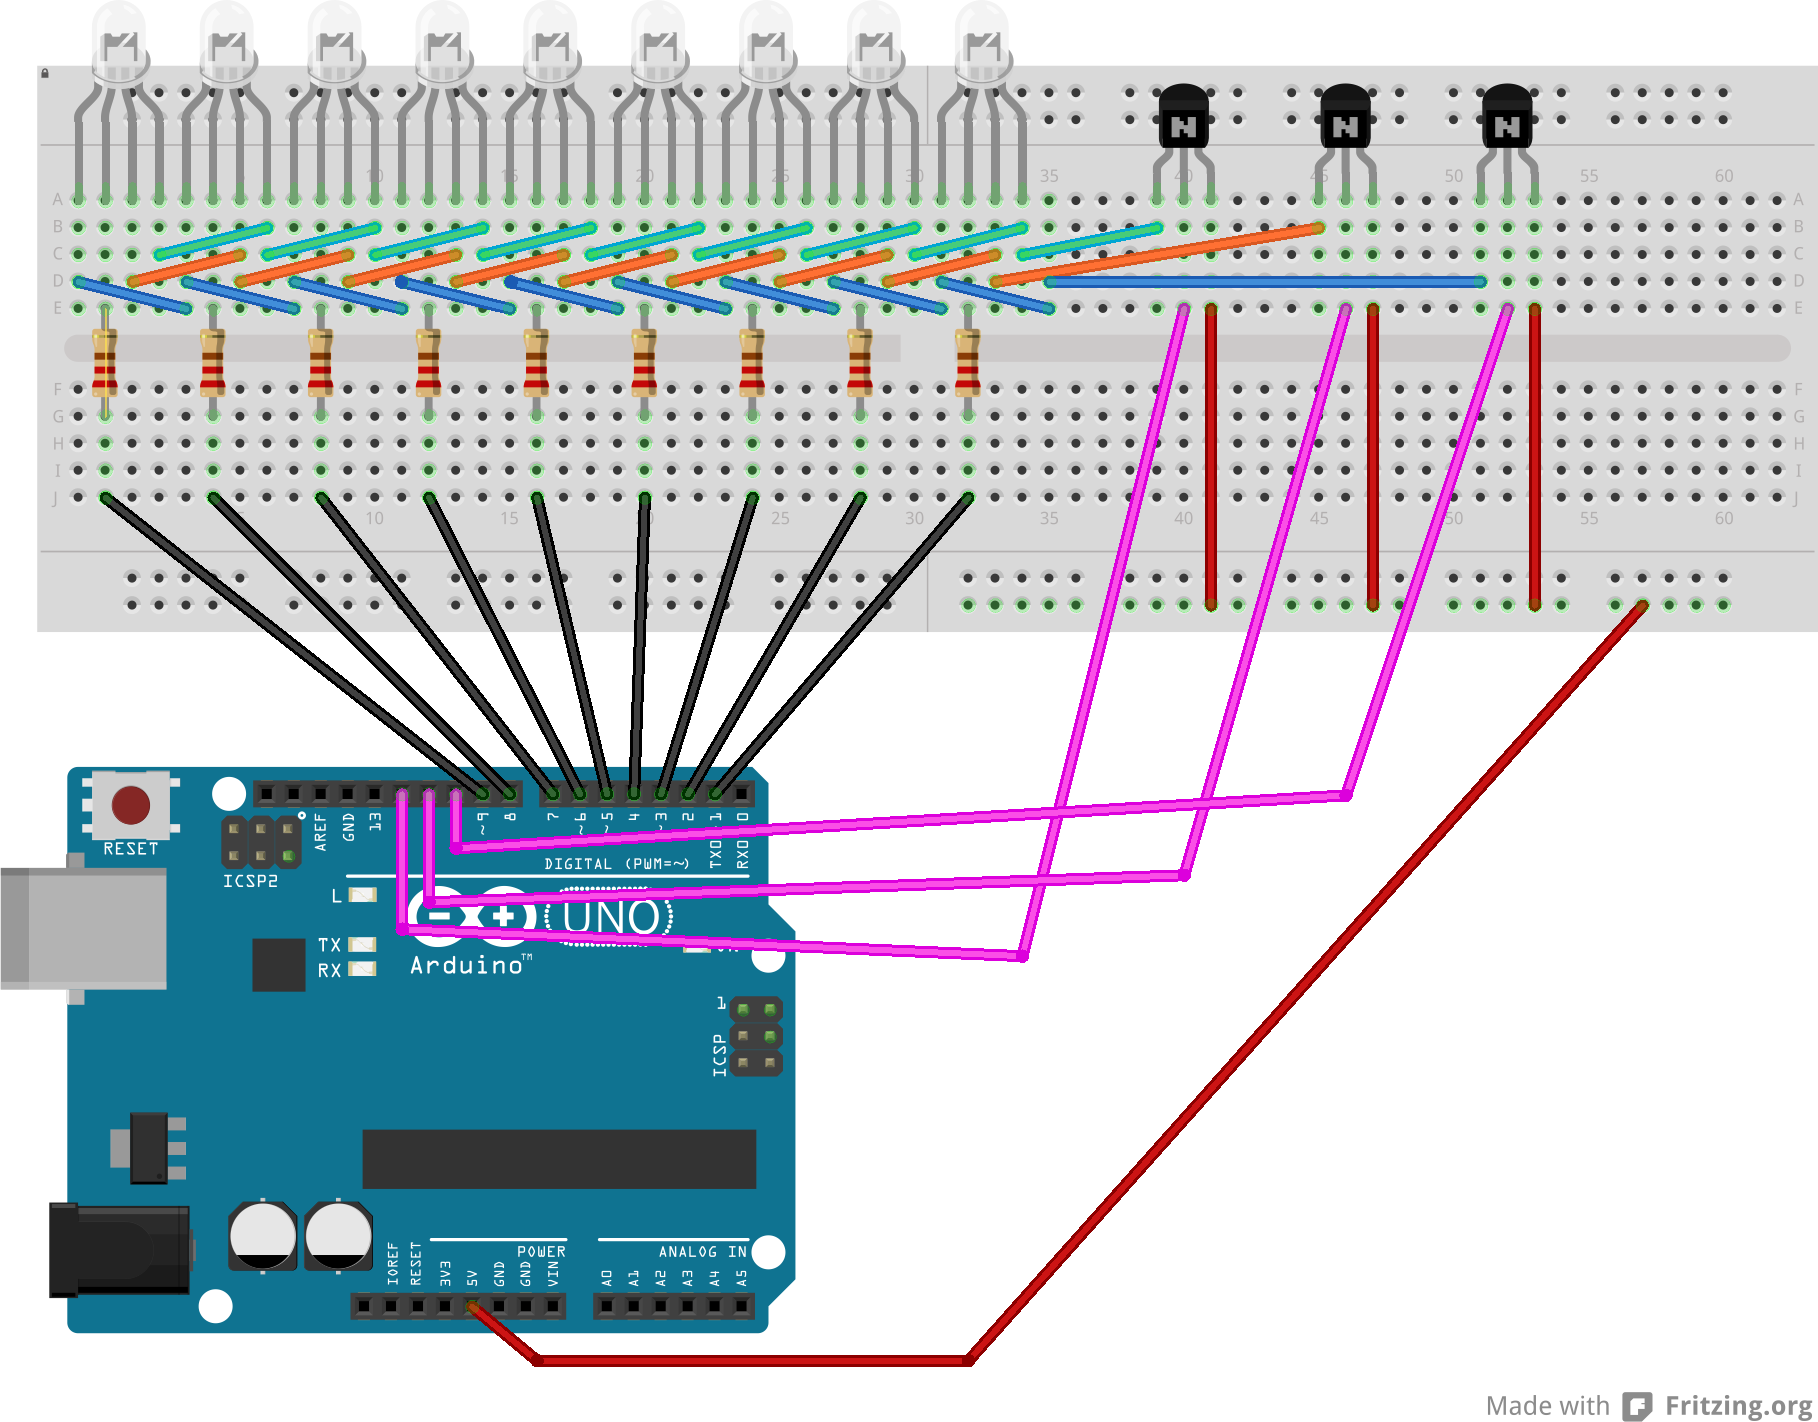
\includegraphics[width=11cm]{img/05_fecube_02_bb.png} 
\caption{\engt{Connect the resistors to pins 1 to 9. The colors go via an npn to the GND (cathode) or 5V (anode). Pins 10, 11, 12 go to the NPN to control the colors.} \nedt{Verbind de weerstanden met pinnen 1 tot 9. De kleuren gaan via een npn naar de GND (kathode) of 5V (anode). Pinnen 10, 11, 12 gaan naar de NPN om de kleuren te schakelen.}}
\label{f:lesson3_bb2}
\end{figure}

\subsection{\engt{Testing breadboard Fe Cube}  \nedt{Schakelbord Fe Cube uittesten}}

\eng{We will only verify we can make the breadboard Fe Cube work. For this we adapt our RGB sketches. We will make a movie showing  4 seconds red, then 4 seconds green, then 4 seconds blue, then 1 minute a random color, then smooth transitions for 1 minute.

This means we need all the shots we created for the RGB LED in the previous lesson, and need to create an adapted \ardo{movie} function to connect the shots as we want. We also need to change the start so that instead of only one led pin, we start up 9 led pins. 

In our previous script, we had ledR, ledG, ledB, which are easy to understand names. The led was called led1, so we could use led1 to led9. This is not very helpfull if you want to program certain light effects. So, let's give them better names. We have a top layer (T), and a bottom (B) layer, and a single LED in the middle. Then we can divide the cube in a left (L) and right (R), and in a front (F) and an aft (A). So, let's call the LEDs:
\begin{enumerate}
\item ledTLF
\item ledTLA
\item ledTRF
\item ledTRA
\item ledBLF
\item ledBLA
\item ledBRF
\item ledBRA
\item ledMID
\end{enumerate}
Open Code \ref{c:l2_d}, and save it under a new name. The changes needed are first defining all the pins:
}

\ned{TODO}

\inputard{\string"../sketches/Fe_cube_03_cube_test1/Fe_cube_03_cube_test1.ino\string"}{5}{11}

\eng{Next we need to define in \ardo{setup} that these are digital output pins, so:}


\ned{TODO}

\inputard{\string"../sketches/Fe_cube_03_cube_test1/Fe_cube_03_cube_test1.ino\string"}{15}{24}

\eng{We test the cube as a single LED, so all LED are on, or all LED are off. Hence, instead of setting only led1 on, we write a function to put all LED on, and put that in \ardo{show\_subframe\_color}}
\ned{TODO}

\inputard{\string"../sketches/Fe_cube_03_cube_test1/Fe_cube_03_cube_test1.ino\string"}{215}{216}

\eng{This new function for setting the pins \textbf{on} sends a LOW signal to the pins, as we are connected to the LED cathode (-)}
\ned{TODO}
\inputard{\string"../sketches/Fe_cube_03_cube_test1/Fe_cube_03_cube_test1.ino\string"}{242}{248}

\eng{Finally, we need to update the \ardo{movie} function so that it would do what we want. So this function needs to be}
\ned{TODO}

\inputard{\string"../sketches/Fe_cube_03_cube_test1/Fe_cube_03_cube_test1.ino\string"}{109}{149}


\engo{\begin{doE}
      \textbf{One LED}. To test that a single LED does indeed not shine brighter when it is alone, change the \ardo{all\_led\_on} code so that only one LED has power.
     \end{doE}
}
\nedo{\begin{doN}
      \textbf{\'E\'en LED}. Om te testen dat een LED alleen inderdaad niet helderder brandt, wijzig de \ardo{all\_led\_on} functie zodat maar \'e\'en LED aan is.
     \end{doN}
}


\subsection{\engt{Construction}  \nedt{Constructie}}
\eng{We verified all is working, time to construct the cube. For this we will take components of our breadboard, and solder the connections in a FE Cube form.
We call our cube the Fe Cube because it is organized as the Iron (Fe) metal lattice. Solid iron has a specific structure which is depicted in the \href{http://en.wikipedia.org/wiki/Atomium}{Atomium building} in Brussels. We call it a \href{http://en.wikipedia.org/wiki/Cubic_crystal_system}{Body-centered cubic crystal system}, short \textbf{bcc}.  This is a cube with an extra node in the center. 


}

\ned{TODO}

\section{\engt{Lesson 4: Fire up the LED Cube} \nedt{Les 4: De LED Cube gebruiken}}

\subsection{\engt{Testing the Fe Cube} \nedt{De Fe Cube testen}}
\eng{You finished now constructing the cube. We need to test if all lights are working. Start with the same sketch you used for the breadboard cube. If you connect everything correctly, it should just work. 

If things are not working, you have some extra soldering to do: replace a blown out LED, make connections stronger, ... . Don't give up now. These are the last construction problems of your led cube.}
\ned{TODO}

\subsection{\engt{Generic patterns ... and a snake} \nedt{Algemene patronen ... en een slang}}

\eng{
We have a working cube now, but we can only show single colors with our current code. Let's change that. We want to be able to write some light effects, and show that on our cube. So let us create a movie function that can load patterns we create. Like that we can write down a pattern, and pass it to this function. The first pattern we want to make is the snake pattern: a single light that jumps from LED to LED in the three base colors.

We need to define the data structure of a pattern. What needs to be in a pattern?
\begin{enumerate}
 \item We need for 9 LED what color they must have. A color is a RGB value like (13,50,2), assuming we still use values between 0 and 64. That is, we need $3\times 9 = 27$ numbers to form a frame now.
 \item We need to know how long to hold a frame before moving to the next frame. So, we need an extra number for the milliseconds, for a total of 28 numbers.
\end{enumerate}
Therefore, a pattern will look like a list of numbers which indicate the different frames and how long they take. For a single frame this will be:\newline
$\{$R1,G1,B1, R2,G2,B2, R3,G3,B3, R4,G4,B4, R5,G5,B5, R6,G6,B6, R7,G7,B7, R8,G8,B8, R9,G9,B9, duration$\}$\newline

The order of the LEDS in the frame will be ledTLF, ledTLA, ledTRF, ledTRA, ledBLF, ledBLA, ledBRF, ledBRA, ledMID. If a shot consists of pattern with 20 fixed frames, we create a single large array with all the frames, one after the other. As Arduino code is not that clever, we need to know somehow what the last pattern is. We could count and pass this number of patterns, but that will quickly lead to an error. Easier is to finish the list with a fake pattern with duration 0. If we read this 0, we know the pattern is finished. 

In our code, our \ardo{movie} function will use a \ardo{moviepattern} function that will handle a pattern you give it. The function will divide the pattern in shots: one shot per fixed frame. The shot will take as long as the duration you have passed in the pattern. This shot is the analogue of the \ardo{fixed\_color} for the single RGB LED: \ardo{fixed\_pattern}, which is a shot that produces a single fixed image on the cube.

There is an extra complication though. The Arduino does not have a lot of memory to work with. There is the SRAM memory with which the Arduino works, and there is Flash memory where your program will be stored. All general variables in your code need to be available at all times, so they need to be stored in SRAM memory. Our patterns can be large though, and the memory would fill up, causing the Arduino to just not produce anything anymore. To avoid this, we will store the patterns in flash memory, and only obtain the frame of the pattern we need. Because of this, you will find in the code:

\textbullet \ \textbf{\#include $<$avr/pgmspace.h$>$}\newline
This will define the functions we need to move data from flash memory to SRAM.

\textbullet \  \textbf{const PROGMEM prog\_int16\_t PatternSnakeRGB{$\lbrack$} {$\rbrack$} = \{ ... \};}\newline

This replaces a normal \textbf{int array{$\lbrack$} {$\rbrack$}} which defines an array of integers. It indicates we want an array of integers, but we want it in \ardo{PROGMEM}, so in the memory that stores our program, the flash memory.

\textbullet You call in the \ardo{movie} function the new \ardo{moviepattern} function if you want to send a pattern to the LED cube. We cannot pass a variable with the moviepattern we want to use because this is now in \ardo{PROGMEM}. You will need to edit \ardo{moviepattern} to load the correct pattern.

\textbullet In the function \ardo{moviepattern} you see twice the appearance of the \ardo{switch} structure. This is a programming structure that works like a switch based on a variable. The syntax is:\newline
 %
\textbf{switch (var) \{ \newline
\ \  case label1:\newline
\ \ \ \     // statements for when var==label1\newline
\ \ \ \     break;\newline
\ \   case label2:\newline
\ \ \ \     // statements for when var==label2\newline
\ \ \ \     break;\newline
  default: \newline
    // statements for if var was something different\newline
\}}\newline
In this switch structure, the commands for which the var is equal to one of the labels are executed from that point onwards, up to a \ardo{break;} command.

In the first switch structure you need to add the start conditions of the patterns you want to show. In the second switch structure you need to copy the pattern you want into the \ardo{shotpattern} variable, as well set the \ardo{nextduration} variable to the duration of the next shot. The function \ardo{pgm_read_word_near} is the function that will copy from the program memory (flash) to SRAM. The only thing needed to change there is the name of the pattern, or add a case with your pattern.

\textbullet \  The start conditions for a pattern are:
\begin{enumerate}
 \item \textbf{patternscale\_start}: with what time scaling to start? This is multiplied with the duration of a frame.
 \item \textbf{patternscale\_speedup}: a value larger than 0 and less than 1. Every time the pattern is finished, you can make it go faster. This speedup is multiplied with the duration of the frames
 \item \textbf{patternscale\_min}: it has no use to go always faster, you need to stop some time. This indicates the minimum scale, after which we assume the pattern can be completely stopped.
 \item \textbf{patternrepeatmin}: as the fastest presentation at patternscale\_min will be so fast you can hardly see it, you can set with this variable how many times to repeat this fastest pattern before we really consider the pattern as finished. When the pattern is finished in this way, the label of the switch command, NRPATTERN in the sketch, is increased by one, causing a next pattern to be loaded if that is present.
 \item \textbf{totalpatterns}: we use the switch command to select the pattern. Give with this variable how many patterns in total you use. 
\end{enumerate}
To show the influence of changing these parameters, the code has an extra pattern called PatternCircle, which uses different starting values.

\textbullet \ The rest of the extra code is to compute the correct speedup of the shots in the pattern, and to determine correctly when a pattern is finished and the next pattern can begin.
}

\ned{TODO}

\eng{
The entire code is given in Code \ref{c:ledcube_snake}.
}

\ned{TODO}

\begin{code}\label{c:ledcube_snake}
 \ \newline
\inputardfull{\string"../sketches/Fe_cube_03_cube_pattern/Fe_cube_03_cube_pattern.ino\string"}
\end{code}


\engo{\begin{doE}
      \textbf{Your pattern}. Time to make your own pattern. How about a rotating emergency vehicle light? Or christmass twinkle? Or ....
     \end{doE}
}
\nedo{\begin{doN}
      \textbf{Jouw patroon}. Tijd om je eigen patroon te maken. Wat denk je van een zwaailicht? Of kerstboom flikkering? Of ...
     \end{doN}
}

\subsection{\engt{Intelligent patterns ... and a beating heart} \nedt{Intelligente patronen ... en een kloppend hart}}

\eng{We can do patterns, which is nice, but patterns are a lot of work to create. This is no different in animation movies or with special effects. They take a lot of time to make. So, people use programming instead to do as much of the work as possible. 

For example, if you look at our snake pattern, we essentially repeat 3 times the same pattern but for a different color. It would be easier to write the pattern once, and then in the code shift the pattern one color. As another example, consider writing a pattern for a beating heart. We would go from no light, to always more red. When all if fully red, we would invert it. In essence, we would need to repeat the pattern in reverse order. Again, with software this would be easier and avoid us writing a long pattern. 

Before writing more software, it is important to design it somewhat. We now end a pattern with a dummy line which has duration 0. As a duration smaller than zero makes no sense, we can use a negative duration to indicate performing a specific operation on the pattern, for example reverse it as in the beating heart, or shift the colors as in the snake. Apart from this, we would need a counter also to indicate how often to extend the pattern once the end is reached. 

We will use following definitions: the variable \ardo{extend_pattern} will contain how often the pattern must be extended when the end is reached. The final duration will indicate how the pattern must be repeated. We will consider as durations
\begin{itemize}
 \item[0]: the pattern does not change. This is the end
 \item[-1]: reverse the pattern in the next repeat
 \item[-11]: shift the colors one to the right: R$\rightarrow$G, G$\rightarrow$B, B$\rightarrow$R
 \item[-12]: shift the colors two to the right: R$\rightarrow$B, G$\rightarrow$R, B$\rightarrow$G
 \item[-90]: rotate the shot over -90 degrees. Ideal to create rotating animations.
 \item[-180]: flip the shot, so TLF becomes TRA
 \item[-270]: rotate the shot over 90 degrees
\end{itemize}

Doing all these changes will increase the amount of code. As our patterns are smaller however, we will be able to do more with less memory.
}

\ned{TODO}

\eng{First, the patterns can be shorter. Here are the two patterns we consider, our snake of before, and the beating heart.}

\ned{TODO}

\inputard{\string"../sketches/Fe_cube_03_cube_intpattern/Fe_cube_03_cube_intpattern.ino\string"}{17}{33}

%\begin{code}\label{c:ledcube_heart}
% \ \newline
%\inputardfull{\string"../sketches/Fe_cube_03_cube_intpattern/Fe_cube_03_cube_intpattern.ino\string"}
%\end{code}

\eng{All the other changes are in our \ardo{moviepattern} function. We have two extra control variables: \ardo{extend_pattern} indicating how many times a single pattern is extended by a copy with some effects on. So, for the original snake, we reduced the 3 loops to one loop in red, so we need to extend it twice to obtain the original length.

The other new variable is \ardo{starteffect}. That is, we need not wait for an extend to apply an effect, we can do it from the start. To show what is possible with effects, we manipulate the red snake pattern in 4 different ways, as well as adding a beating heart pattern. The adapted \ardo{moviepattern} function is
}
\ned{}

\inputard{\string"../sketches/Fe_cube_03_cube_intpattern/Fe_cube_03_cube_intpattern.ino\string"}{147}{297}


\engo{\begin{doE}
      \textbf{More patterns}. The effects are working? Add another effect, eg a color change. Or just write a new pattern using some of the effects.
     \end{doE}
}
\nedo{\begin{doN}
      \textbf{Meer patronen}. De effecten werken op je Fe Kubus? Voeg een nieuw effect toe, bevoorbeeld een kleurverandering. Of schrijf gewoon een nieuw patroon dat van enkele effecten gebruik maakt.
     \end{doN}
}


\section{\engt{Lesson 4: Interaction with a push button: Dices} \nedt{Les 4: Interactie met een drukknop: Dobbelstenen}}

\eng{TODO}
\ned{Je kan prachtige dingen doen met je kubus. Maar we kunnen het nog wat gebruiksvriendelijker maken. Ware het niet super als je kon interageren met je kubus. Bevoorbeeld van effect veranderen als je een knop drukt? Of je kubus omtoveren in een dobbelsteen die je rolt als je op de knop drukt.}

\subsection{\engt{How does a pushbutton work?} \nedt{Hoe werkt een drukknop?}}

